\chapter{Diseño y Construcción del Gabinete de Control (Prototipo)}
\lineaLateral
\begin{resumenCapitulo}
Se describe el proceso de diseño, dimensionamiento y ensamblaje del gabinete de control. Esta etapa de prototipado es fundamental para validar la distribución espacial de los componentes electrónicos, la gestión de conexiones y las necesidades de ventilación antes de la fabricación del chasis final.
\end{resumenCapitulo}

\section{Lista de materiales}
\begin{itemize}
	\item Madera MDF de 15 mm de ancho
	\item Madera MDF de 10 mm de ancho
	\item Flexómetro
	\item Router
	\item Sierra de inglete
	\item Sacabocado para madera
	\item Taladro, brocas, tornillos
\end{itemize}

\section{Dimensionamiento y Diseño en SolidWorks}

El diseño del gabinete se originó en la plataforma CAD \textit{SolidWorks}, permitiendo un modelado preciso de los componentes críticos como la fuente de poder, los controladores BTS7960, la barra de bus, el regulador de voltaje, el sistema de ventilación y el Arduino Mega. 

En esta etapa de prototipado, se dio prioridad a la construcción de un chasis funcional para mitigar el riesgo operativo de conectar y desconectar el cableado de potencia y control de manera constante, lo cual suele derivar en fatiga de materiales o errores de conexión. Asimismo, este enfoque permitió validar de forma empírica la distribución espacial de los módulos y la gestión del flujo de aire, asegurando que la arquitectura interna responda eficientemente a las necesidades de disipación térmica y accesibilidad antes de proceder a la manufactura del gabinete final.

\begin{figure}[h]
	\centering
	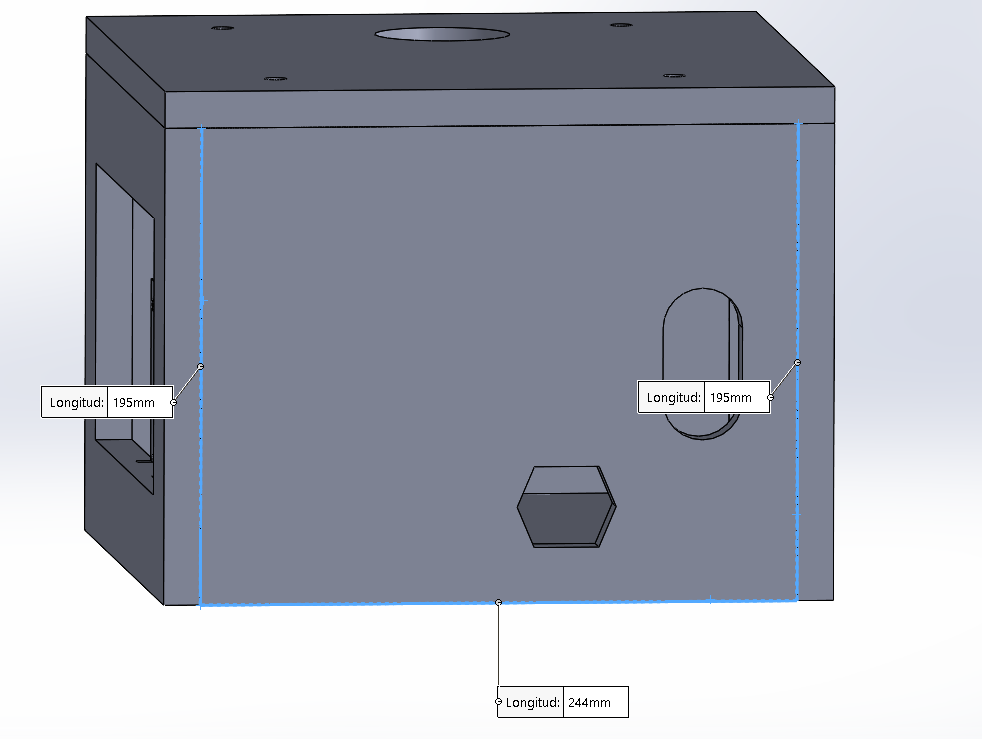
\includegraphics[width=0.7\linewidth]{images/Enclosure/screenshot022}
	\caption[Pieza frontal de la caja.]{Vista frontal del gabinete de control. Se observa el mecanizado para la interfaz de conexión del brazo robótico (señales de encoders y frenos) y una cavidad hexagonal diseñada para el montaje de una base de enchufe tipo industrial, funcionando como terminal de alimentación principal. Mide 244 x 195 mm.}
	\label{fig:screenshot022}
\end{figure}

\begin{figure}[h]
	\centering
	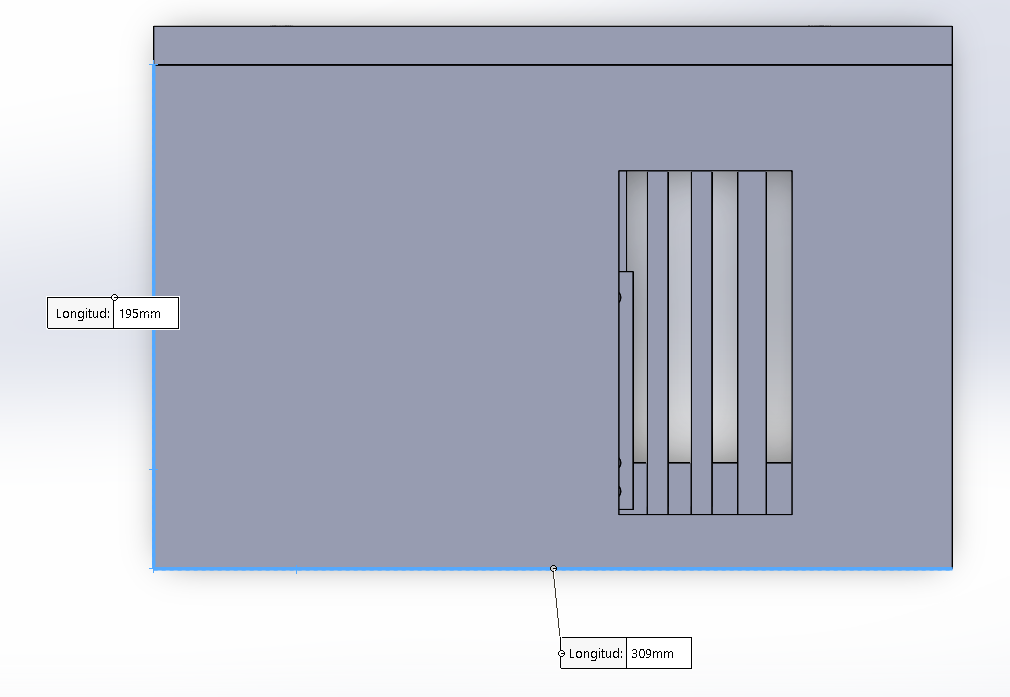
\includegraphics[width=0.7\linewidth]{images/Enclosure/screenshot023}
	\caption[Pieza lateral derecha del gabinete.]{Vista lateral derecha del gabinete donde se aprecian las ranuras de ventilación pasiva. Estas aberturas han sido dimensionadas para permitir un flujo de aire entrante constante, optimizando la eficiencia del ventilador interno en la extracción de calor y manteniendo los componentes electrónicos dentro de su rango térmico de operación. Mide 309 x 195 mm.}
	\label{fig:screenshot023}
\end{figure}

\begin{figure}[h]
	\centering
	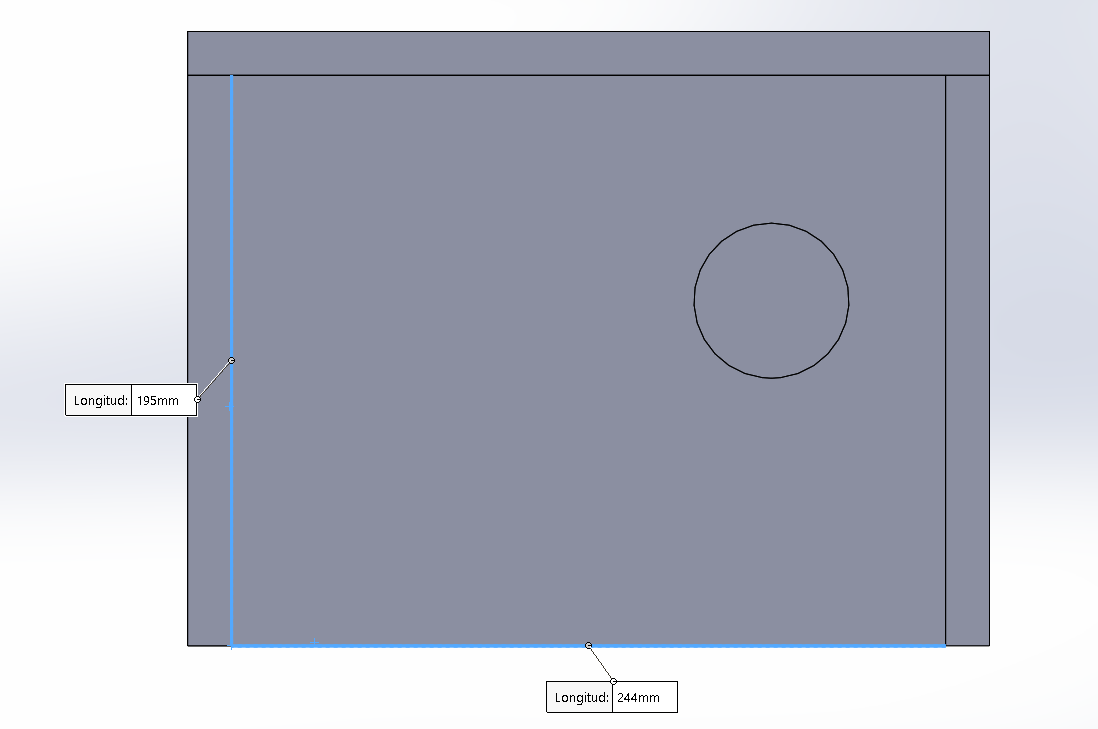
\includegraphics[width=0.7\linewidth]{images/Enclosure/screenshot024}
	\caption[Pieza posterior de la caja,]{Vista posterior del gabinete de control. Se presenta la cavidad circular mecanizada para coincidir con la salida de aire de la fuente de poder interna. Este diseño permite la expulsión de aire caliente hacia el exterior protegiendo así la integridad de la electrónica de control. Mide 244 x 195 mm.}
	\label{fig:screenshot024}
\end{figure}

\begin{figure}[h]
	\centering
	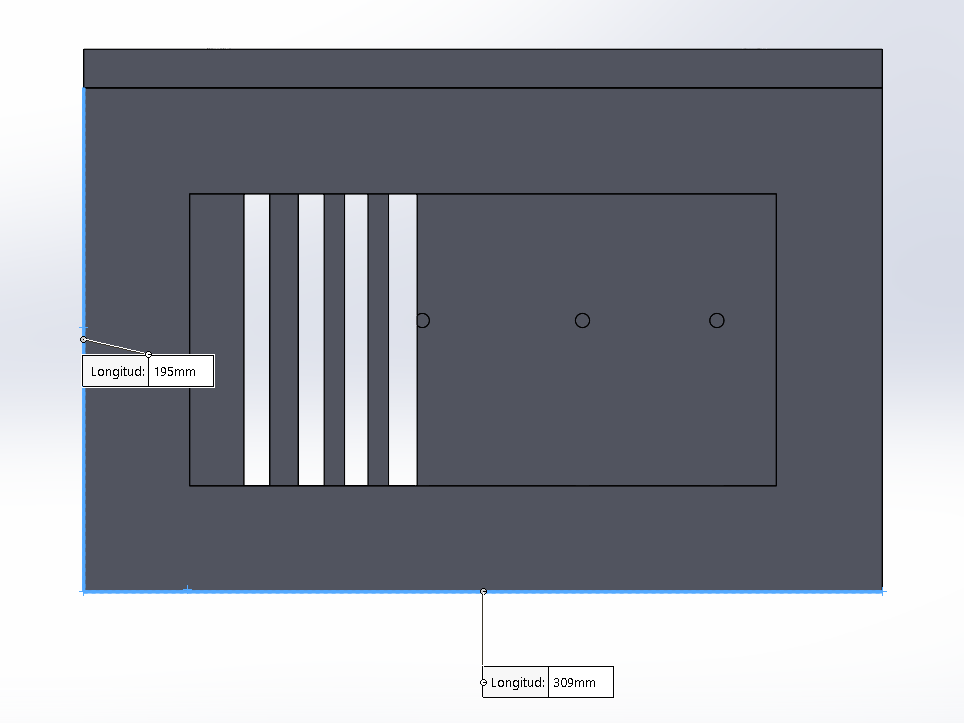
\includegraphics[width=0.7\linewidth]{images/Enclosure/screenshot025}
	\caption[Pieza lateral izquierda del gabinete]{Panel lateral izquierdo del gabinete. Se ha integrado una ventana de acrílico transparente que permite la supervisión visual directa de la arquitectura interna, facilitando el monitoreo de las repisas de soporte y el estado operativo de los componentes electrónicos sin comprometer el aislamiento del gabinete. Mide 309 x 195 mm.}
	\label{fig:screenshot025}
\end{figure}

\begin{figure}[h]
	\centering
	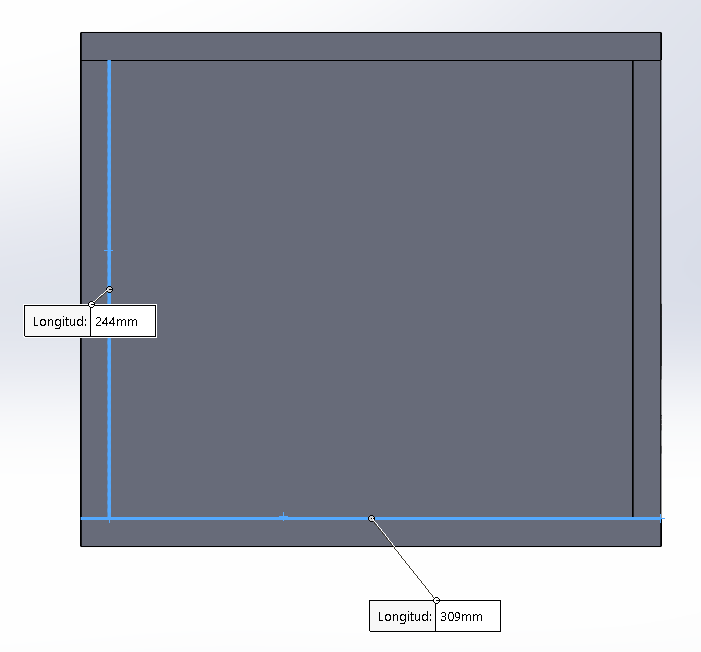
\includegraphics[width=0.7\linewidth]{images/Enclosure/screenshot026}
	\caption[Pieza base del gabinete.]{Pieza base del gabinete. Mide 309 x 244 mm.}
	\label{fig:screenshot026}
\end{figure}

\begin{figure}[h]
	\centering
	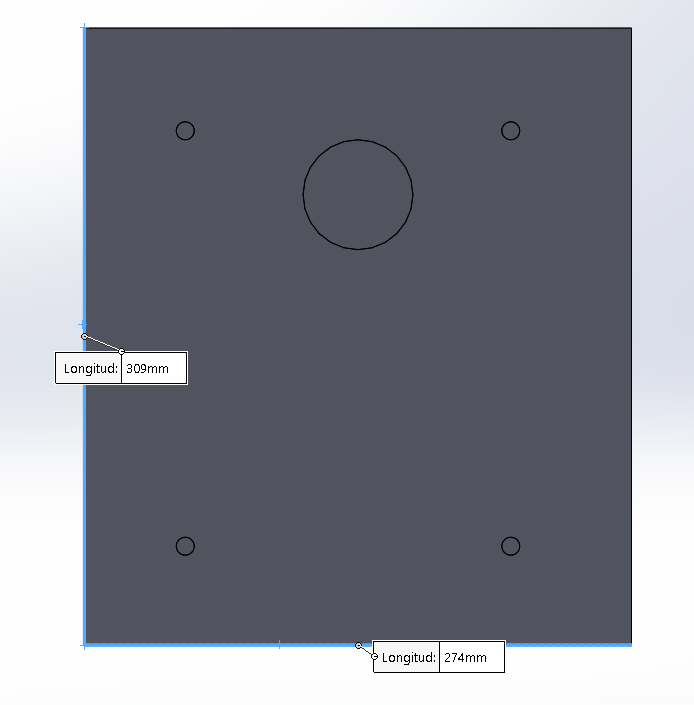
\includegraphics[width=0.7\linewidth]{images/Enclosure/screenshot027}
	\caption[Pieza superior del gabinete]{Vista superior del gabinete de control. Esta pieza cumple la función de base estructural, integrando barrenos de sujeción reforzados para el anclaje del brazo robótico. Asimismo, cuenta con una cavidad para un ventilador de extracción, diseñado para forzar la salida del aire caliente generado por la electrónica interna. Mide 247 x 309 mm.}
	\label{fig:screenshot027}
\end{figure}

\begin{figure}[h]
	\centering
	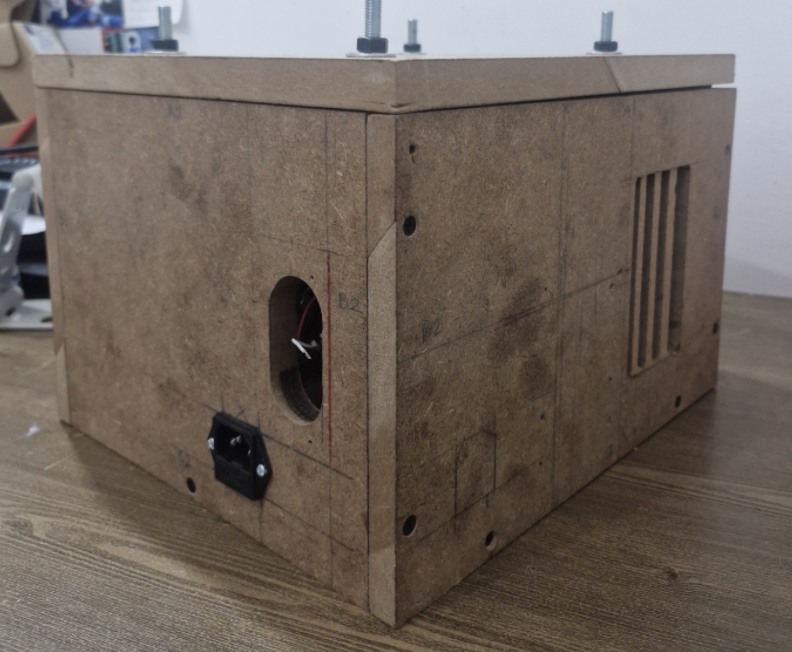
\includegraphics[width=0.7\linewidth]{images/Enclosure/screenshot028}
	\caption[Vista de la caja desde la esquina frontal derecha]{Vista de la caja desde la esquina frontal derecha.}
	\label{fig:screenshot028}
\end{figure}

\begin{figure}[h]
	\centering
	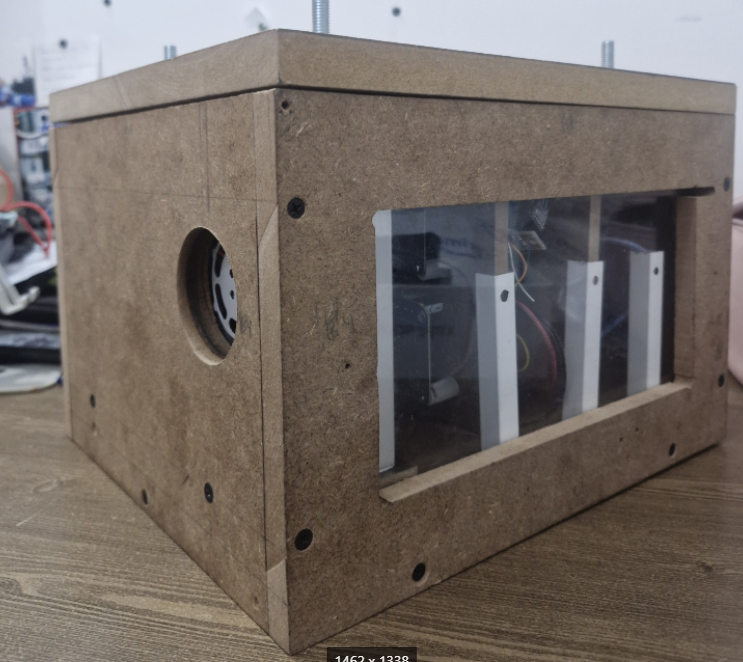
\includegraphics[width=0.7\linewidth]{images/Enclosure/screenshot029}
	\caption[Vista del gabinete desde la cara trasera]{Vista del gabinete desde la cara trasera.}
	\label{fig:screenshot029}
\end{figure}


\clearpage
\section{Arquitectura Interna y Distribución de Repisas}
% Describe la organización por niveles.
La distribución interna del gabinete se proyectó bajo criterios de organización lógica y facilidad de mantenimiento. Se optó por una configuración de repisas dispuestas de manera perpendicular al plano de la ventana de acrílico, lo que permite una inspección visual de todos los niveles desde el exterior. 

Para facilitar el acceso a la electrónica, se instalaron guías metálicas atornilladas a las paredes laterales del chasis. Este mecanismo permite que las repisas funcionen como bandejas extraíbles, posibilitando el retiro individual de cada sección (potencia o control) sin necesidad de desensamblar la estructura.   


\begin{figure}[h]
	\centering
	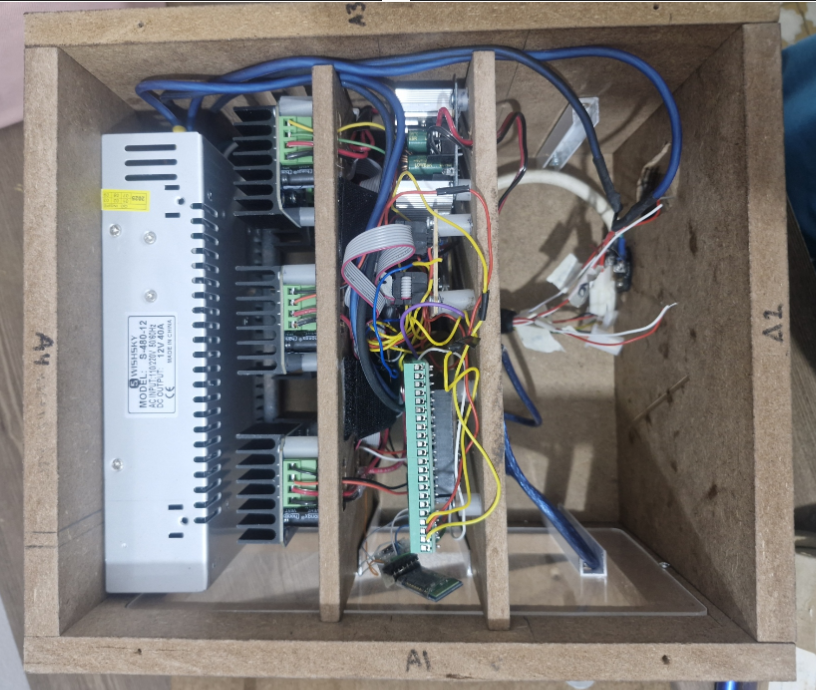
\includegraphics[width=0.85\linewidth]{images/Enclosure/screenshot030}
	\caption[Vista superior de las repisas del gabinete]{Vista superior de las repisas del gabinete. La primera repisa consta de solamente los drivers Bts7960; mientras que la segunda, contiene el arduino Mega, el módulo Bluethooth, regulador de voltaje y una unidad central donde se dirigen las señales del Bts7960 hacia el Arduino Mega.}
	\label{fig:screenshot030}
\end{figure}

\begin{figure}[h]
	\centering
	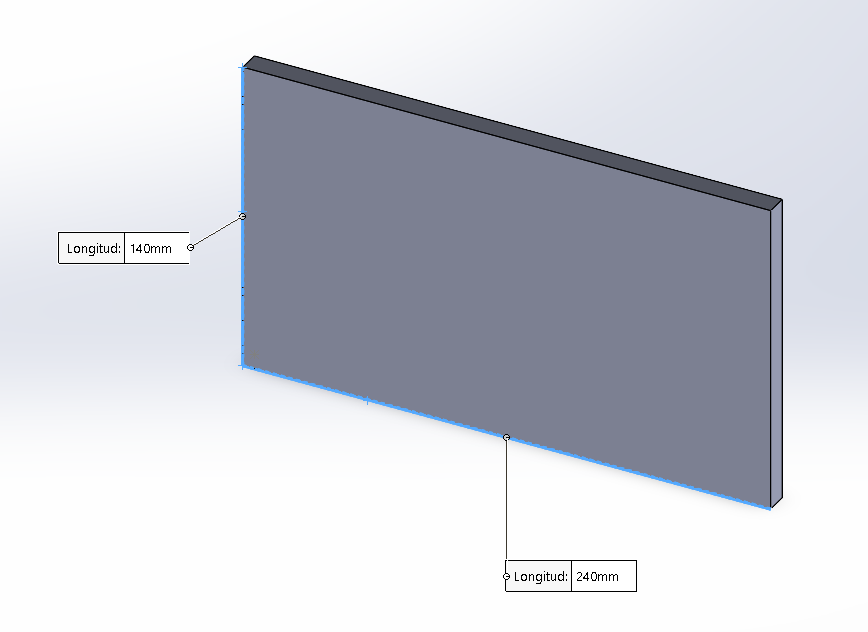
\includegraphics[width=0.7\linewidth]{images/Enclosure/screenshot033}
	\caption[Dimensiones de las repisas]{Medida de las repisas. Fueron de 240 x 140 mm.}
	\label{fig:screenshot033}
\end{figure}


\begin{figure}[h]
	\centering
	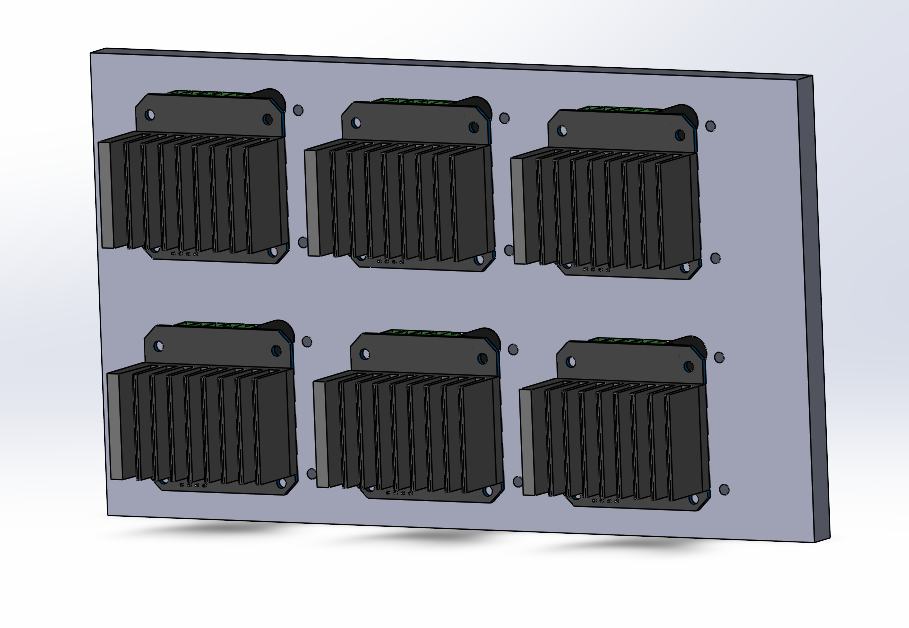
\includegraphics[width=0.7\linewidth]{images/Enclosure/screenshot031}
	\caption[Repisa de los drivers Bts7960]{Primera repisa. Se encuentran conectados los 6 drivers Bts7960 que manejan los motores del brazo robótico.}
	\label{fig:screenshot031}
\end{figure}

\begin{figure}[h]
	\centering
	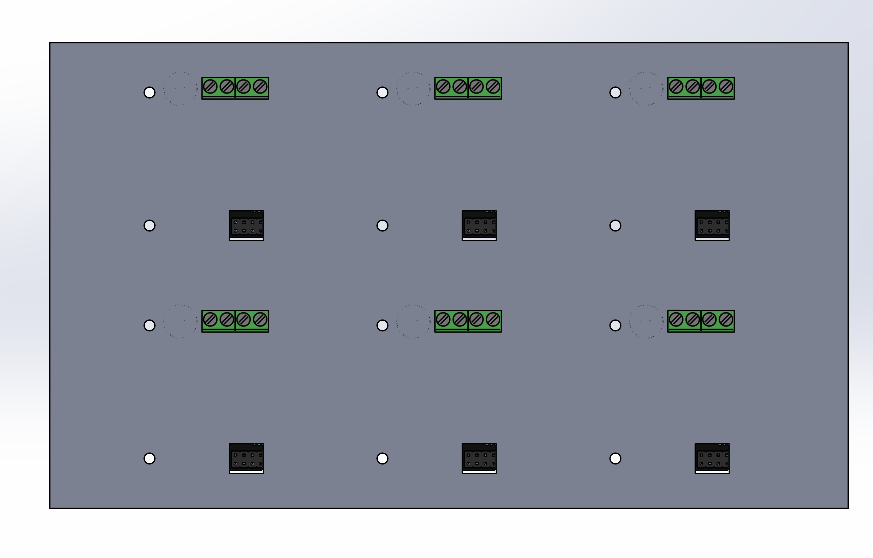
\includegraphics[width=0.7\linewidth]{images/Enclosure/screenshot032}
	\caption[Vista trasera de la repisa de los drivers Bts7960]{Vista trasera de la repisa de los drivers Bts7960, contiene accesos hacia los tornillos de las borneras y conexión a los pines del driver Bts7960.}
	\label{fig:screenshot032}
\end{figure}

\begin{figure}[h]
	\centering
	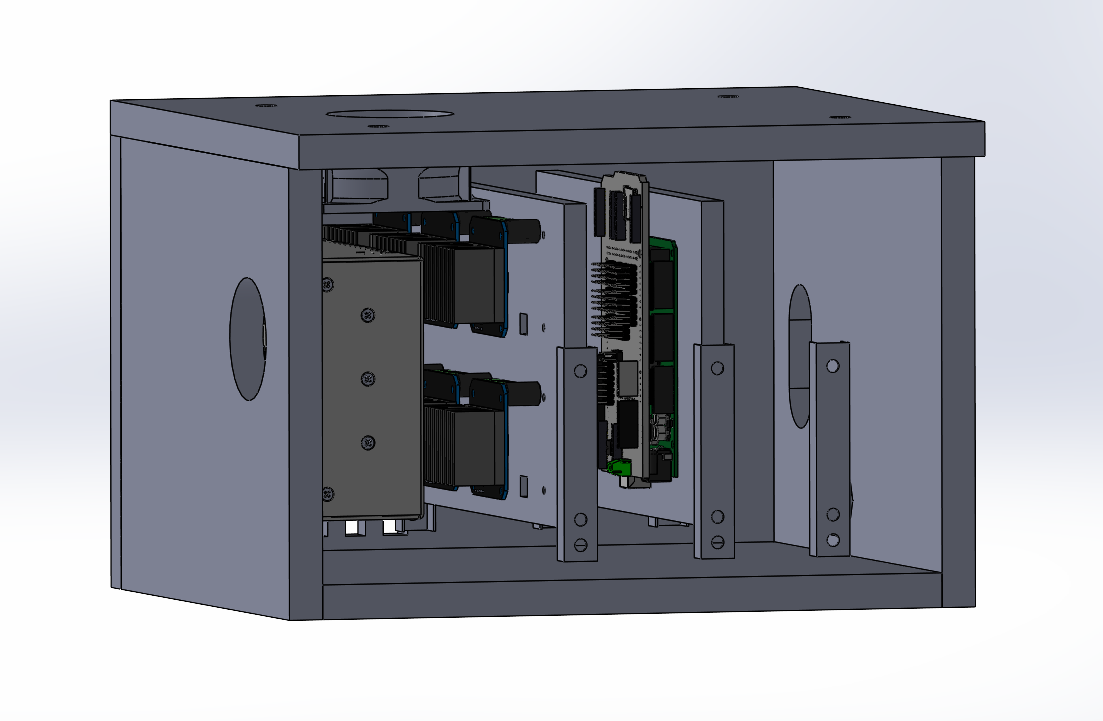
\includegraphics[width=0.7\linewidth]{images/Enclosure/screenshot036}
	\caption{Ensamblaje de los componentes electrónicos en el gabinete.}
	\label{fig:screenshot036}
\end{figure}

\clearpage
\section{Necesidades Técnicas: Ventilación y Pasacables}
% Describe los huecos que mencionaste.
A partir de la disposición física, se identificaron las necesidades de mecanizado para el gabinete:
\begin{itemize}
	\item \textbf{Ventilación:} Localización de huecos para ventiladores activos que mitiguen el calor generado por los puentes H.
	\item \textbf{Interfaz Externa:} Espacios dedicados para el conector de alimentación de $127\,V_{CA}$ y la salida de los puertos que se conectan a los motores.
\end{itemize}

\begin{figure}[ht]
	\centering
	% Imagen de la izquierda
	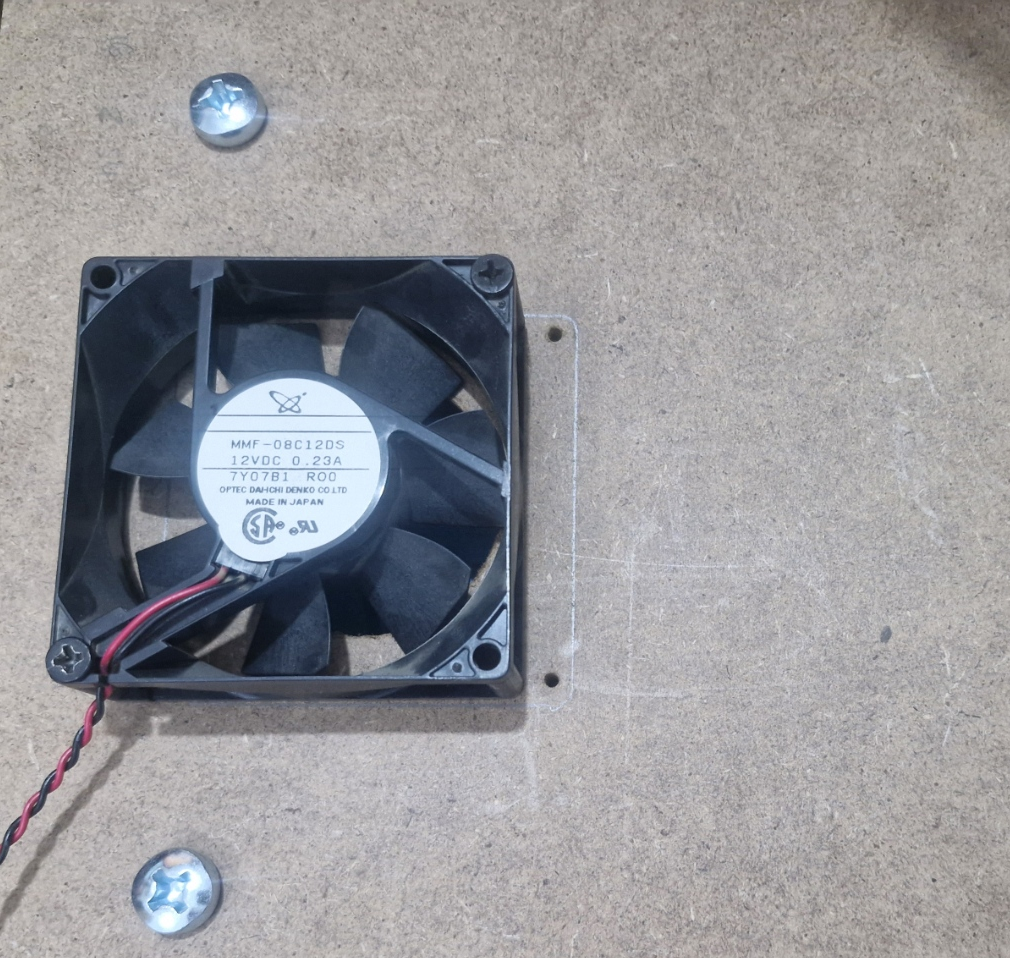
\includegraphics[width=0.45\linewidth]{images/Enclosure/screenshot034}
	\hspace{0.5cm} % Espacio horizontal entre imágenes
	% Imagen de la derecha
	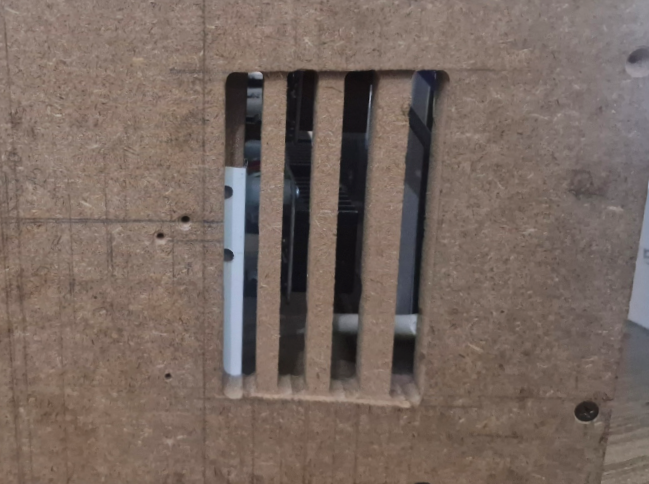
\includegraphics[width=0.45\linewidth]{images/Enclosure/screenshot035}
	
	\caption[Ventilación del gabinete]{Sistema de ventilación: extractor de aire caliente (izquierda) y rendijas de entrada de aire (derecha).}
	\label{fig:ventilacion_sistema}
\end{figure}


\section{Análisis de Mejoras para el Gabinete Final}

A partir de la experiencia obtenida con la fabricación y el ensamble de este primer prototipo, se han identificado puntos críticos que permitirán optimizar la versión final del gabinete de control. Las mejoras propuestas se enfocan en la mantenibilidad, la robustez de las conexiones y la miniaturización del sistema:

\begin{itemize}
	\item \textbf{Reorientación de Repisas:} Se plantea cambiar la disposición de las repisas de vertical a horizontal. Se detectó que la configuración actual complica el paso de cables entre niveles; al posicionarlas horizontalmente, se facilita el acceso y la organización del cableado.
	\item \textbf{Interconexión Modular:} Para mejorar el sistema de bandejas extraíbles, cada nivel contará con una PCB dedicada que centralice las señales. Se propone el uso de conectores de tipo aviador (roscados), permitiendo que para retirar una repisa solo sea necesario desenchufar o desenroscar los conectores, eliminando la necesidad de manipular cables sueltos.
	\item \textbf{Optimización del Cableado:} Se planea sustituir los cables de los buses de potencia por trayectorias más cortas para reducir caídas de tensión. Asimismo, se reemplazarán los alambres rígidos por cable flexible, ya que el alambre tiende a desconectarse o fracturarse con el movimiento y la manipulación de las repisas.
	\item \textbf{Mecanizado de Repisas:} Se rediseñarán los huecos de acceso en las repisas de los \textit{drivers} BTS7960. En el prototipo actual, el espacio es reducido, lo que dificulta la inserción de los cables en las borneras. Los nuevos barrenos serán más amplios para facilitar el uso de herramientas.
	\item \textbf{Miniaturización y Comunicación:} Se evaluará la sustitución del Arduino Mega por una tarjeta de desarrollo más compacta que mantenga la capacidad de procesamiento necesaria. Además, se reubicará el módulo Bluetooth en una posición más accesible o cercana a las paredes externas para mejorar la calidad de la señal y facilitar el emparejamiento.
	\item \textbf{Actualización de PCBs:} Se rediseñarán las placas de circuito impreso para integrar mejor los conectores de aviador y optimizar el ruteo de las señales de los sensores ACS712, reduciendo el ruido electromagnético.
\end{itemize}

\clearpage
\begin{resultadosFase}
	\begin{itemize}
		\item \textbf{Portabilidad del sistema:} Se logró concentrar toda la electrónica de control y potencia en una sola unidad compacta, lo que facilita el transporte del sistema sin riesgo de dañar los componentes o perder la configuración del cableado.
		\item \textbf{Claridad en las conexiones:} El diseño de la cara frontal y la organización interna permitieron que las conexiones hacia el brazo robótico (motores y encoders) sean mucho más ordenadas y fáciles de identificar, reduciendo errores humanos durante el ensamble.
		\item \textbf{Optimización del espacio:} La fabricación del gabinete permitió entender de forma práctica la distribución real que requieren los módulos BTS7960, la fuente y el Arduino, validando que el diseño modular por repisas es una solución efectiva para aprovechar el volumen interno.
		\item \textbf{Validación del sistema térmico:} Se confirmó que la ubicación de las ranuras de ventilación y los ventiladores de extracción son suficientes para mantener un flujo de aire constante, evitando el sobrecalentamiento de los controladores bajo carga de trabajo.
		\item \textbf{Identificación de necesidades críticas:} Esta fase permitió descubrir la importancia de utilizar cables flexibles y conectores más robustos, así como la necesidad de ampliar los accesos a las borneras para facilitar el mantenimiento.
		\item \textbf{Protección del hardware:} Se consiguió un entorno seguro para la electrónica, aislándola de agentes externos y proporcionando una base sólida y estable para el anclaje mecánico del brazo robótico.
	\end{itemize}
\end{resultadosFase}